\documentclass[Dissertation.tex]{subfiles} 
\begin{document}

\chapter{The Bound State: Positronium Hydride}
\label{chp:PsHBound}

\lettrine{\textcolor{startcolor}{A}}{s} discussed in \cref{sec:PsH}, positronium hydride consists of one atom of positronium and one of hydrogen. We model it the standard way here as an exotic atom, instead of a molecule. \Cref{fig:PsHCoords} shows the PsH coordinate system. There are 6 interparticle coordinates, given by $r_1$, $r_2$, $r_3$, $r_{12}$, $r_{13}$, and $r_{23}$. The proton is considered infinitely heavy in this treatment.

\begin{figure}[!h]
	\centering
	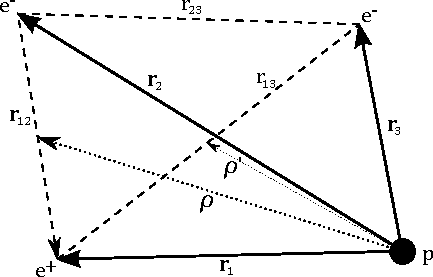
\includegraphics[height=3in]{PsHCoordinates}
	\caption{Positronium hydride coordinate system}
	\label{fig:PsHCoords}
\end{figure}

\section{Positronium Hydride (PsH) Wavefunction}
\label{sec:BoundWavefn}

\textbf{@TODO:} Write what $P_{23}$ is and why we need it (indistinguishable electrons).

Our wavefunction for the bound state is a Hylleraas-style set of terms, given by
\begin{subequations}
\label{eq:BoundWavefn}
\begin{align}
\Psi^\pm &= \sum_{i=1}^{N(\omega)} c_i \bar{\phi}_i^\pm \label{eq:BoundWavefn_psi} \\
\bar{\phi}_i^\pm &= (1 \pm P_{23}) \phi_i \label{eq:BoundWavefn_phibar} \\
\phi_i &= e^{-(\alpha r_1 + \beta r_2 + \gamma r_3)} r_1^{k_i} r_2^{l_i} r_{12}^{m_i} r_3^{n_i} r_{13}^{p_i} r_{23}^{q_i} \label{eq:BoundWavefn_phi} \, ,
\end{align}
\end{subequations}
where the plus sign indicates the spatially symmetric singlet case, and the minus sign indicates the spatially antisymmetric triplet case. The permutation operator $P_{23}$ is needed, as the two electrons are indistinguishable. The $\frac{1}{\sqrt{2}}$ needed %for \textbf{@TODO: Why exactly? Flux?}%
to normalize $\Psi^\pm$ (to cancel out the 2 in \cref{eq:RRfinal}) is absorbed into the $c_i$ constant in equation \ref{eq:BoundWavefn_psi}. The constant $\SphericalHarmY{0}{0}{\theta}{\phi} = \frac{1}{\sqrt{4\pi}}$ is also absorbed into $c_i$.
% For clarity in some equations, the definition $d_i = \frac{1}{\sqrt{4\pi}} c_i$ is used.

The variable $\omega$ is an integer $\geq 0$ that determines the number of terms in the basis set.  For a chosen value of $\omega$, the integer powers of $r_i$ and $r_{ij}$ are constructed in such a way that
\beq
\label{eq:OmegaDef}
k_i + l_i + m_i + n_i + p_i + q_i \leq \omega
\eeq
\noindent with all $k_i$, $l_i$, $m_i$, $n_i$, $q_i$ and $p_i$ $\geq 0$.  Using combination with repetition, an explicit formula for $N(\omega)$ is given as

\beq
\label{eq:NumberTermsOmega}
N(\omega) = \Binomial{\omega+6}{6} \, ,
\eeq
\noindent where the 6 comes from the 6 coordinates of $r_i$ and $r_{ij}$.  A plot of $N(\omega)$ versus $\omega$ is given in \cref{fig:NOmega}.

\begin{figure}[H]
	\centering
	%\scalebox{1}{\includegraphics{NOmega}}
	\includegraphics[width=4in]{NOmega}
	\caption{$N(\omega)$ versus $\omega$}
	\label{fig:NOmega}
\end{figure}


\section{Rayleigh-Ritz Variational Method}
The Rayleigh-Ritz variational method is given as the functional \cite{Bransden2003}
\beq
\label{eq:RayleighRitz}
E[\Psi] = \frac{\Braket{\Psi | H | \Psi}}{\Braket{\Psi | \Psi}}.
\eeq

\noindent This provides an upper bound to the ground-state energy, $E_0$.  In other words,
\beq
E_0 \leq E[\Psi].
\eeq
This can be rewritten in matrix notation as a generalized eigenvalue problem \cite{RayleighRitz}
\beq
\label{eq:BoundGenEig}
\textbf{Hc} = E\textbf{Sc},
\eeq
where
\beq
\label{eq:HijSij}
H_{ij} = \left< \bar{\phi}_i \left| H \right| \bar{\phi}_j \right>\!, \, S_{ij} = \left< \bar{\phi}_i \left| \right.\! \bar{\phi}_j \right>, 
\eeq
and \textbf{c} is the vector of coefficients for the wavefunction $\Psi$.  The normalization here is unimportant due to the division in equation \ref{eq:RayleighRitz} and the form of equation \ref{eq:BoundGenEig}.

For PsH, the non-relativistic Hamiltonian is
\beq
\label{eq:BoundHamiltonian}
H = -\frac{1}{2} \nabla_{r_1}^2 - \frac{1}{2} \nabla_{r_2}^2 - \frac{1}{2} \nabla_{r_3}^2 + \frac {1}{r_1}-\frac {1}{r_2}-\frac {1}{r_3}-\frac {1}{r_{12}}-\frac {1}{r_{13}}+\frac {1}{r_{23}}.
\eeq

The Laplacians in equation \ref{eq:BoundHamiltonian} are complicated when applied to the $\phi_j$ function.  We exploit the short-range nature of $\phi_i$ and $\phi_j$ by using integration by parts, similar to equation (3.21) of Armour and Humberston \cite{Armour1991}.
\beq
\label{eq:BoundGradient}
-\Int{ \phi_i \left(\nabla_{r_1}^2 + \nabla_{r_2}^2 + \nabla_{r_3}^2 \right) \phi_j }{\tau} = \int \sum_{l=1}^3 \bm{\nabla}_{\!\bm{r}_l} \phi_i \bm{\cdot} \bm{\nabla}_{\!\bm{r}_l} \phi_j \, d\tau
\eeq

\noindent This expression is simpler than applying the Laplacian operators directly to $\phi_j$, and the summation is given by the following expression (a full derivation is given on the research Wiki \cite{Wiki}):

\begin{align}
\nonumber \sum_{l=1}^3 \bm{\nabla}_{\!\mathbf{r}_l} \phi_i \bm{\cdot} \bm{\nabla}_{\!\mathbf{r}_l} \phi_j = &\phi_i \phi_j \Bigg\{(\alpha^2 + \beta^2 + \gamma^2) - \frac{\alpha}{r_1}(k_i + k_j) - \frac{\beta}{r_2}(l_i + l_j) + \frac{\gamma}{r_3}(n_i + n_j) \\
\nonumber  &+ \frac{k_i k_j}{r_1^2} + \frac{l_i l_j}{r_2^2} + \frac{n_i n_j}{r_3^2} + \frac{2 m_i m_j}{r_{12}^2} + \frac{2 p_i p_j}{r_{13}^2} + \frac{2 q_i q_j}{r_{23}^2} \\
\nonumber  &+ \frac{r_1^2 + r_{12}^2 - r_2^2}{2 r_1^2 r_{12}^2} \left[-\alpha r_1(m_i+m_j) + (k_i m_j + k_j m_i)\right] \\
\nonumber  &+ \frac{r_1^2 + r_{13}^2 - r_3^2}{2 r_1^2 r_{13}^2} \left[-\alpha r_1(p_i+p_j) + (k_i p_j + k_j p_i)\right] \\
\nonumber  &+ \frac{r_{12}^2 + r_{13}^2 - r_{23}^2}{2 r_{12}^2 r_{13}^2} \left[m_i p_j + m_j p_i\right] \\
\nonumber  &+ \frac{r_2^2 + r_{12}^2 - r_1^2}{2 r_2^2 r_{12}^2} \left[-\beta r_2(m_i+m_j) + (m_i l_j + m_j l_i)\right] \\
\nonumber  &+ \frac{r_2^2 + r_{23}^2 - r_3^2}{2 r_2^2 r_{23}^2} \left[-\beta r_2(q_i+q_j) + (l_i q_j + l_j q_i)\right] \\
\nonumber  &+ \frac{r_{12}^2 + r_{23}^2 - r_{13}^2}{2 r_{12}^2 r_{23}^2} \left[m_i q_j + m_j q_i\right] \\
\nonumber  &+ \frac{r_3^2 + r_{13}^2 - r_1^2}{2 r_3^2 r_{13}^2} \left[-\gamma r_3(p_i+p_j) + (n_i p_j + n_j p_i)\right] \\
\nonumber  &+ \frac{r_3^2 + r_{23}^2 - r_2^2}{2 r_3^2 r_{23}^2} \left[-\gamma r_3(q_i+q_j) + (n_i q_j + n_j q_i)\right] \\
		   &+ \frac{r_{13}^2 + r_{23}^2 - r_{12}^2}{2 r_{13}^2 r_{23}^2} \left[p_i q_j + p_j q_i\right] \Bigg\}.
\end{align}

The full expression for $H_{ij}$ from equation \ref{eq:HijSij} after using \cref{eq:BoundHamiltonian,eq:BoundGradient} is then
\beq
\label{eq:BoundHFull}
\left< \bar{\phi}_i \left| H \right| \bar{\phi}_j \right> = \Int{ \left[ \frac{1}{2}\sum_{l=1}^3 \boldsymbol{\nabla}_{\!\mathbf{r}_l} \bar{\phi}_i \boldsymbol{\cdot} \boldsymbol{\nabla}_{\!\mathbf{r}_l} \bar{\phi}_j + \left( \frac {1}{r_1}-\frac {1}{r_2}-\frac {1}{r_3}-\frac {1}{r_{12}}-\frac {1}{r_{13}}+\frac {1}{r_{23}} \right) \bar{\phi}_i \bar{\phi}_j \right]}{\tau}.
\eeq

To reduce the number of integrations needed by half, we use a property of the permutation operator.  Since 
\beq
\left< \phi_i \left| H \right| \phi_j \right> = \left< P_{23} \phi_i \left| H \right| P_{23} \phi_j \right>
\eeq
and
\beq
\left< \phi_i \left| H \right| P_{23} \phi_j \right> = \left< P_{23} \phi_i \left| H \right| \phi_j \right>,
\eeq
expression \ref{eq:BoundHFull} becomes
\begin{subequations}
\begin{align}
\nonumber \left< (1 \pm P_{23}) \phi_i \left| H \right| (1 \pm P_{23}) \phi_j \right> =& \left< \phi_i \left| H \right| \phi_j \right> \pm \left< P_{23} \phi_i \left| H \right| \phi_j \right> \\
&\pm \left< \phi_i \left| H \right| P_{23} \phi_j \right> + \left< P_{23} \phi_i \left| H \right| P_{23} \phi_j \right> \\
=& 2 \left[ \left< \phi_i \left| H \right| \phi_j \right> \pm \left< P_{23} \phi_i \left| H \right| \phi_j \right> \right] \\
=& 2 \left[ \left< \phi_i \left| H \right| \phi_j \right> \pm \left< \phi_i \left| H \right| P_{23} \phi_j \right> \right]
\end{align}
\end{subequations}



%\subsection{Energy Derivatives}
\section{Parameter Optimization}
\label{sec:BoundOpt}
The most powerful property of the Rayleigh-Ritz variational method is the ability to systematically improve the wavefunction to lower the upper bound on the energy. By either adding terms to the expansion in \ref{eq:BoundWavefn_psi} or changing the nonlinear parameters $\alpha$, $\beta$ and $\gamma$, the energy can be reduced and a possible minimum found. This is a three-dimensional optimization problem, and we tried multiple methods for the nonlinear parameter optimization.

\subsection{Newton's Method}

\subsubsection{Energy Derivatives}
\label{sec:EnergyDer}
\textbf{@TODO:} Start with mention of Drake/Yan paper.

\beq
\Psi = \sum_{i=1}^N c_i \psi_i
\eeq

\textbf{Rewrite parts of this in terms of formulas in BoundState.tex.}

The variational method gives
\beq
E = \frac{\left< \Psi \left| H \right| \Psi \right>}{\left< \Psi \left| \right.\! \Psi \right>}
  = \frac{\displaystyle\sum_{i=1}^N \sum_{j=1}^N \left< c_i \psi_i \left| H \right|  c_j \psi_j \right>}{\displaystyle\sum_{i=1}^N \sum_{j=1}^N \left<c_i \psi_i \left| \right.\! c_i \psi_i \right>}
  = \frac{\displaystyle\sum_i \sum_j c_i^* c_j H_{ij}}{\displaystyle\sum_i \sum_j c_i^* c_j S_{ij}} \equiv \frac{A}{B}
\eeq

where
\beq
H_{ij} = \left< \psi_i \left| H \right| \psi_j \right>
\text{ and }
S_{ij} = \left< \psi_i \left| \right.\! \psi_j \right>.
\eeq

$\dfrac{\partial A}{\partial c_k^*}$ or $\dfrac{\partial B}{\partial c_k^*}$ will reduce the double summation to a single sum, since 
$ \dfrac{\partial c_i^*}{\partial c_k^*} =
\begin{cases}
1,& i = k \\
0,& i \neq k
\end{cases}.$

To minimize the energy, $E$,
\beq
\label{eq:RRfinal}
\frac{\partial E}{\partial c_k^*} = \frac{\partial A}{\partial c_k^*} \frac{1}{B} - \frac{1}{B^2} \frac{\partial B}{\partial c_k^*} A
= \frac{1}{B} \left(\frac{\partial A}{\partial c_k^*} - E \frac{\partial B}{\partial c_k^*}\right)
= \frac{\displaystyle\sum_{j=1}^N (H_{kj} - E S_{kj})}{B} = 0.
\eeq

We want to minimize the energy with respect to the nonlinear parameters $\alpha, \beta$ and $\gamma$.  Let us concern ourselves with the $\alpha$ parameter:  $\Psi = \Psi(\alpha, ...)$.

\beq
\frac{\partial E}{\partial \alpha} = \frac{1}{B} \left(\frac{\partial A}{\partial \alpha} - E \frac{\partial B}{\partial \alpha} \right)
\label{eq:EnergyDerE1}
\eeq

Since $\alpha$ is real, $\alpha^* = \alpha$.  Our wavefunction is real as well, i.e. $\Psi^* = \Psi$.  The Hamiltonian, H, is independent of $\alpha$ and is Hermitian, so
\beq
\frac{\partial A}{\partial \alpha} = \left< \Psi \Big| H \Big| \frac{\partial\Psi}{\partial \alpha} \right> + 
    \left< \frac{\partial\Psi}{\partial \alpha} \Big| H \Big| \Psi \right> = 2 \left< \Psi \Big| H \Big| \frac{\partial\Psi}{\partial \alpha} \right>
\label{eq:EnergyDerPartA}
\eeq
\beq
\frac{\partial B}{\partial \alpha} = \left< \Psi \Big| \frac{\partial\Psi}{\partial \alpha} \right> + 
    \left< \frac{\partial\Psi}{\partial \alpha} \Big| \Psi \right> = 2 \left< \Psi \Big| \frac{\partial\Psi}{\partial \alpha} \right>
\label{eq:EnergyDerPartB}
\eeq

Combining (\ref{eq:EnergyDerPartA}) and (\ref{eq:EnergyDerPartB}) with (\ref{eq:EnergyDerE1}) gives
\beq
\frac{\partial E}{\partial \alpha} = \frac{2 \left< \Psi \Big| H \Big| \frac{\partial\Psi}{\partial \alpha} \right> - 2 \left< \Psi \Big| \frac{\partial\Psi}{\partial \alpha} \right>}{\left< \Psi \Big| \Psi \right>}.
\label{eq:EnergyDerivative}
\eeq

\noindent If $\Psi$ is properly normalized, $\left< \Psi \Big| \Psi \right> = 1$, the simplified version can be used:
\beq
\frac{\partial E}{\partial \alpha} = 2 \left< \Psi \Big| H \Big| \frac{\partial\Psi}{\partial \alpha} \right> - 2 \left< \Psi \Big| \frac{\partial\Psi}{\partial \alpha} \right>.
\label{eq:EnergyDerivativeNorm}
\eeq

\noindent This is the form given in Drake and Yan \cite{Drake1995}.

Similar forms for the other parameters are found by replacing $\alpha$ with the parameter of interest.


\subsubsection{Newton's Method}
The derivative with respect to the parameter $\alpha$ can be used with Newton's Method to find a minimum energy.  From \cite{Sauer2006}, Newton's method is given as
\beq
x_{i+1} = x_i - \frac{f(x_i)}{f'(x_i)}.
\label{eq:NewtonMethod}
\eeq

We are looking for roots of the equation $\displaystyle\frac{\partial E}{\partial \alpha} = 0$ to minimize the energy.  From (\ref{eq:NewtonMethod}), $\displaystyle\frac{\partial^2 E}{\partial^2 \alpha}$ is required.  The secant method, a variation of Newton's method, is used to avoid this problem.  From \cite{Sauer2006},
\beq
x_{i+1} = x_i - \frac{f(x_i)(x_i - x_{i-1})}{f(x_i) - f(x_{i-1})}.
\eeq

\noindent The difficulty with this method is that two starting guesses are required, versus the one for Newton's method.


\subsubsection{Singlet Wavefunction Derivatives}
Taking the derivative with respect to $\alpha$ of equation \ref{eq:BoundWavefn_psi} yields
\beq
\frac{\partial \Psi^+}{\partial \alpha} = \sum_i c_i \frac{\partial \phi_i}{\partial \alpha} = \sum_i c_i (1+P_{23}) \frac{\partial \phi_i}{\partial \alpha} = -r_1 \Psi^{(+)}.
\label{eq:PsiDerAlpha}
\eeq

The $\beta$ and $\gamma$ cases are similar, but the presence of the $P_{23}$ permutation operator complicates the derivative slightly.
\begin{align}
\nonumber \frac{\partial \Psi^{(+)}}{\partial \beta} &= \sum_i c_i \frac{\partial}{\partial \beta} \left[(1+P_{23}) \phi_i \right] \\
\nonumber &= \sum_i c_i \left\{
  e^{-\alpha r_1} r_1^{k_i} \frac{\partial}{\partial \beta}
  \left[e^{-(\beta r_2 + \gamma r_3)} r_2^{l_i} r_{12}^{m_i} r_3^{n_i} r_{13}^{p_i} r_{23}^{q_i}
      + e^{-(\beta r_3 + \gamma r_2)} r_3^{l_i} r_{13}^{m_i} r_2^{n_i} r_{12}^{p_i} r_{23}^{q_i} \right] \right\} \\
\nonumber &= \sum_i c_i \left(
  e^{-(\alpha r_1 + \gamma r_3)} r_1^{k_i} r_2^{l_i} r_{12}^{m_i} r_3^{n_i} r_{13}^{p_i} r_{23}^{q_i} \frac{\partial}{\partial \beta} e^{-\beta r_2} +
  e^{-(\alpha r_1 + \gamma r_2)} r_1^{k_i} r_3^{l_i} r_{13}^{m_i} r_2^{n_i} r_{12}^{p_i} r_{23}^{q_i} \frac{\partial}{\partial \beta} e^{-\beta r_3} \right) \\
 &= \sum_i c_i \left(-r_2 \phi_i - r_3 P_{23} \phi_i \right) 
\label{eq:PsiDerBeta}
\end{align}

Likewise,
\beq
\frac{\partial \Psi^{(+)}}{\partial \gamma} = \sum_i c_i \left(-r_3 \phi_i - r_2 P_{23} \phi_i \right)
\label{eq:PsiDerGamma}
\eeq


\subsubsection{Triplet Wavefunction Derivatives}
Similar calculations for the triplet give

\begin{align}
\frac{\partial \Psi^{(-)}}{\partial \alpha} &= -r_1 \Psi^{(-)} \label{eq:PsiTripletDerAlpha} \\
\frac{\partial \Psi^{(-)}}{\partial \beta} &= \sum_i c_i \left(-r_2 \phi_i + r_3 P_{23} \phi_i \right) \label{eq:PsiTripletDerBeta} \\
\frac{\partial \Psi^{(-)}}{\partial \gamma} &= \sum_i c_i \left(-r_3 \phi_i + r_2 P_{23} \phi_i \right) \label{eq:PsiTripletDerGamma}
\end{align}


\subsection{Results of Nonlinear Parameter Optimization}

For the results in table \ref{table:NonlinearOptimized1SNewton}, starting guesses were $\alpha = 0.6$, $\beta = 0.6$ and $\gamma = 1.0$.  The value of $h \equiv x_i - x_{i-1}$ was chosen to be $10^{-5}$.  We also examined different starting guesses, which gave similar results but took more steps to reach them.


\setlength{\abovecaptionskip}{6pt}   % 0.5cm as an example
\setlength{\belowcaptionskip}{6pt}   % 0.5cm as an example
\begin{table}[ht]
\caption{Newton Optimized Singlet Nonlinear Parameters} % title of Table
\centering
\begin{tabular}{c c c c}
\hline\hline
$\omega$ & $\alpha$ & $\beta$ & $\gamma$ \\ [0.5ex]
\hline
1 & 0.53604 & 0.59507 & 1.02169 \\
2 & 0.57424 & 0.65051 & 0.98174 \\
3 & 0.58945 & 0.62992 & 0.97556 \\
4 & 0.58490 & 0.60928 & 0.98691 \\
5 & 0.58004 & 0.59303 & 1.01069 \\
\hline\hline
\end{tabular}
\label{table:NonlinearOptimized1SNewton}
\end{table}


\subsection{Broyden's Method}
The above analysis used the 1-dimensional Newton's method and changed each nonlinear parameter separately.  This worked well for the singlet but became a problem for the calculations involving the triplet state.  The code for optimization was modified to use Broyden's method \cite{Sauer2006}, which can solve for all three nonlinear parameters simultaneously.  Newton's method for n-dimensions can be used as well, though it requires computation of the Jacobian.

The three equations in (\ref{eq:PsiDerAlpha})-(\ref{eq:PsiDerGamma}) or (\ref{eq:PsiTripletDerAlpha})-(\ref{eq:PsiTripletDerGamma}) can be solved in the three unknowns $\alpha$, $\beta$ and $\gamma$ by Broyden's method.  The second Broyden's method, sometimes referred to as the ``bad Broyden's method'' was used here.  As Kvaalen points out, this method is perfectly usable and can be faster than the first Broyden's method \cite{Kvaalen1991}.


\setlength{\abovecaptionskip}{6pt}   % 0.5cm as an example
\setlength{\belowcaptionskip}{6pt}   % 0.5cm as an example
\begin{table}[ht]
\caption{Broyden Optimized Singlet Nonlinear Parameters} % title of Table
\centering
\begin{tabular}{c c c c}
\hline\hline
$\omega$ & $\alpha$ & $\beta$ & $\gamma$ \\ [0.5ex]
\hline
1 & 0.535920 & 0.594515 & 1.022061 \\
2 & 0.571412 & 0.598429 & 1.056740 \\
3 & 0.535149 & 0.620153 & 1.120099 \\
4 & 0.583859 & 0.592326 & 1.016347 \\
5 & 0.530239 & 0.627306 & 1.127732 \\
6 & 0.533933 & 0.632110 & 1.132448 \\
\hline\hline
\end{tabular}
\label{table:NonlinearOptimized1SBroyden}
\end{table}


\setlength{\abovecaptionskip}{6pt}   % 0.5cm as an example
\setlength{\belowcaptionskip}{6pt}   % 0.5cm as an example
\begin{table}[ht]
\caption{Old Broyden Optimized Triplet Nonlinear Parameters} % title of Table
\centering
\begin{tabular}{c c c c}
\hline\hline
$\omega$ & $\alpha$ & $\beta$ & $\gamma$ \\ [0.5ex]
\hline
1 & 0.264440 & 0.831645 & 0.498871 \\
2 & 0.356175 & 0.452426 & 0.829591 \\
3 & 0.347611 & 0.467298 & 0.814971 \\
4 & 0.323300 & 0.333783 & 0.974653 \\
5 & 0.303696 & 0.309673 & 0.980637 \\
\hline\hline
\end{tabular}
\label{table:NonlinearOptimized3SBroydenoLD}
\end{table}

\setlength{\abovecaptionskip}{6pt}   % 0.5cm as an example
\setlength{\belowcaptionskip}{6pt}   % 0.5cm as an example
\begin{table}[ht]
\caption{Broyden Optimized Triplet Nonlinear Parameters} % title of Table
\centering
\begin{tabular}{c c c c}
\hline\hline
$\omega$ & $\alpha$ & $\beta$ & $\gamma$ \\ [0.5ex]
\hline
1 & 0.297493 & 0.287209 & 0.996888 \\
2 & 0.329662 & 0.346790 & 0.983649 \\
3 & 0.336829 & 0.350035 & 0.978465 \\
4 & 0.322670 & 0.330642 & 0.984957 \\
5 & 0.310486 & 0.322063 & 0.911863 \\
6 & 0.283810 & 0.287592 & 0.977710 \\
\hline\hline
\end{tabular}
\label{table:NonlinearOptimized3SBroyden}
\end{table}

\subsection{Choice of Nonlinear Parameters}
\subsubsection{Bound and S-Wave}
For the S-wave singlet, to compare directly with Van Reeth's previous calculations \cite{VanReeth2003}, we used $\alpha = 0.5$, $\beta = 0.6$ and $\gamma = 1.1$.  These values are close to the optimized nonlinear parameters found in table \ref{table:NonlinearOptimized1SBroyden}.  The initial guess trials of $\alpha = 0.6$, $\beta = 0.6$ and $\gamma = 1.0$ were also tried, but this lead to difficulties when extrapolating the phase shifts.

We had considerably more difficulty with linear dependence for the S-wave triplet.  To try to circumvent some of the linear dependence problems, we chose $\alpha = 0.323$, $\beta = 0.334$ and $\gamma = 0.975$ from table \ref{table:NonlinearOptimized3SBroyden} for $\omega = 4$.  This set of nonlinear parameters is different from the set that Van Reeth used of $\beta = 0.4$ and $\gamma = 0.8$ \cite{VanReeth2003}.




\section{Program}



\section{Stabilization}
\begin{figure}[ht]
	\centering
	\scalebox{1.3}{\includegraphics[height=3in]{Stabilization}}
	\caption{Stabilization}
	\label{fig:Stabilization}
\end{figure}



\section{Our Results}
\subsection{Bound State: Singlet}

\begin{table}[H]
\begin{center}
\begin{tabular}{|c|c|c|c|c|c|}
\hline
Description & $\alpha$, $\beta$ and $\gamma$ & $\omega$ & N($\omega$) & Used terms & Energy\\
\hline
Double, $10^{-7}$?, with asymptotic expansion & 0.6, 0.6, 1.0 & 6 & 924 & 916 & -0.7891695098 \\
Double, $10^{-7}$?, with asymptotic expansion & 0.6, 0.6, 1.0 & 7 & 1716 & 1585 & -0.7891895683 \\
Double, $10^{-7}$?, with asymptotic expansion & 0.6, 0.6, 1.0 & 8 & 3003 & 1925 & -0.7891945593 \\
Quadruple, $10^{-6}$, with asymptotic expansion & 0.6, 0.6, 1.0 & 8 & 3003 & 2067 & -0.7891945847\\
Double, $10^{-7}$?, with asymptotic expansion & 0.6, 0.6, 1.0 & 9 & 5005 & 2155 & -0.7891958600 \\
\rowcolor{LightCyan}
Double, $10^{-7}$?, with asymptotic expansion & 0.6, 0.6, 1.0 & 10 & 8008 & 2205 & -0.7891963235 \\

Double, $10^{-7}$?, with asymptotic expansion & 0.58, 0.6, 1.0 & 9 & 5005 & 2166 & -0.7891958308\\
Double, $10^{-7}$?, with asymptotic expansion & 0.58, 0.6, 1.0 & 11 & 12376 & 1674 & -0.7891961505\\

Double, $10^{-7}$, with asymptotic expansion & 0.5, 0.6, 1.1 & 6 & 924 & 924 & -0.7891619764\\
Double, $10^{-7}$, without asymptotic expansion & 0.5, 0.6, 1.1 & 6 & 924 & 924 & -0.7891619769\\
\rowcolor{LightCyan}
Double, $10^{-6}$, with asymptotic expansion & 0.5, 0.6, 1.1 & 7 & 1716 & 1608 & -0.7891870914\\
Double, $10^{-6}$, without asymptotic expansion & 0.5, 0.6, 1.1 & 7 & 1716 & 1658 & -0.7891870935\\
Quadruple, $10^{-6}$, with asymptotic expansion & 0.5, 0.6, 1.1 & 7 & 1716 & 1661 & -0.7891870935\\
Double, $10^{-6}$, with asymptotic expansion & 0.5, 0.6, 1.1 & 8 & 3003 & 1653 & -0.7891935019\\
Double, $10^{-6}$, without asymptotic expansion & 0.5, 0.6, 1.1 & 8 & 3003 & 1403 & -0.7891932577\\
Quadruple, $10^{-6}$, with asymptotic expansion & 0.5, 0.6, 1.1 & 8 & 3003 & 1619 & -0.7891934661\\
\hline
\end{tabular}
\caption{Bound State Energy for Singlet PsH}
\label{tab:BoundSingletResults}
\end{center}
\end{table}

The PsH bound state energy code was run for several sets of nonlinear parameters and increasing values of $\omega$.  Some runs were also performed using quadruple precision, but the results for that are preliminary at this point.  Table \ref{tab:BoundSingletResults} contains the results of these runs.  One criteria of Todd's method (\ref{sec:ToddBound}) is that the eigenvalues from the upper and lower triangular matrices must differ by no more than a threshold value.  This threshold is given in the first column.

The best run is given by the first highlighted row, with $\omega = 10$.  We performed a run for $\omega = 11$, but linear dependence issues caused it to returned only 1674 terms, less than the 2205 for $\omega = 10$.  The energy is also higher, so $\omega = 10$ is the practical limit for our calculations without improvements in the code to solve the generalized eigenvalue problem (\ref{eq:BoundGenEig}).  The scattering problem is much more demanding with regards to computation time and linear dependence, so the current set of short-range terms that we use is denoted by the second highlighted row with $\omega = 7$.  

\textbf{@TODO:} Further discussion on the linear dependence in another section


\section{Results}
\subsection{Bound State: Singlet}

\setlength{\abovecaptionskip}{6pt}   % 0.5cm as an example
\setlength{\belowcaptionskip}{6pt}   % 0.5cm as an example
\begin{table}[H]
\centering
\begin{tabular}{c c c c c c c}
\toprule
$\omega$ & Terms & $\alpha$ & $\beta$ & $\gamma$ & Total Energy (au) & Binding Energy (eV) \\ [0.5ex]
\midrule
0 & 1 & 0.60 & 0.60 & 1.00 & -0.541 492 378 889 & --- \\
1 & 7 & 0.60 & 0.60 & 1.00 & -0.744 334 244 165 & --- \\
2 & 28 & 0.60 & 0.60 & 1.00 & -0.778 357 106 972 & 0.771 636 156 726 \\
3 & 84 & 0.60 & 0.60 & 1.00 & -0.786 807 448 395 & 1.001 581 651 009 \\
4 & 210 & 0.60 & 0.60 & 1.00 & -0.788 685 563 109 & 1.052 687 753 648 \\
5 & 462 & 0.60 & 0.60 & 1.00 & -0.789 082 645 582 & 1.063 492 917 716 \\
6 & 916 & 0.60 & 0.60 & 1.00 & -0.789 169 509 836 & 1.065 856 614 384 \\
7 & 1585 & 0.60 & 0.60 & 1.00 & -0.789 189 568 390 & 1.066 402 435 425 \\
8 & 1925 & 0.60 & 0.60 & 1.00 & -0.789 194 559 324 & 1.066 538 245 640 \\
9 & 2166 & 0.60 & 0.60 & 1.00 & -0.789 195 830 870 & 1.066 572 846 182 \\
10 & 2205 & 0.60 & 0.60 & 1.00 & -0.789 196 323 586 & 1.066 586 253 647 \\
11 & 1674 & 0.58 & 0.60 & 1.00 & -0.789 196 284 600 & 1.066 585 192 793 \\
\bottomrule
\end{tabular}
\caption{Ground state energy of positronium hydride} % title of Table
\label{tab:BoundEnergyOld}
\end{table}

The original double precision PsH code was run for a simple choice of the nonlinear parameters $\alpha$, $\beta$ and $\gamma$. During these initial runs, LAPACK returned valid energies through $\omega = 5$. With the $\omega = 6$ runs, it had trouble using the full 924 terms, with \texttt{dsygv} giving an error. Using Todd's algorithm (\cref{sec:ToddBound}), this code returned a usable 916 terms for $\omega = 6$, as given in \cref{tab:BoundEnergyOld}. The original code worked well through $\omega = 10$, but going from $\omega = 9$ to $\omega = 10$ only added an additional 39 terms. The run for $\omega = 11$ was obviously a problem, since it gave less terms than $\omega = 10$ and a higher energy, even when changing the $\alpha$ parameter slightly.

\setlength{\abovecaptionskip}{6pt}   % 0.5cm as an example
\setlength{\belowcaptionskip}{6pt}   % 0.5cm as an example
\begin{table}[H]
\centering
\begin{tabular}{c c c c c c c}
\toprule
$\omega$ & Terms & $\alpha$ & $\beta$ & $\gamma$ & Dissociation Energy (au) & Binding Energy (eV) \\ [0.5ex]
\midrule
0 & 1 & 0.586 & 0.580 & 1.093 & -0.558 977 058 051 & --- \\
1 & 7 & 0.586 & 0.580 & 1.093 & -0.744 698 936 920 & --- \\
2 & 28 & 0.586 & 0.580 & 1.093 & -0.778 246 602 473 & 0.768 629 176 247 \\
3 & 84 & 0.586 & 0.580 & 1.093 & -0.786 743 703 126 & 0.999 847 053 924 \\
4 & 210 & 0.586 & 0.580 & 1.093 & -0.788 672 801 036 & 1.052 340 479 962 \\
5 & 462 & 0.586 & 0.580 & 1.093 & -0.789 082 645 582 & 1.063 460 197 197 \\
6 & 924 & 0.586 & 0.580 & 1.093 & -0.789 169 509 836 & 1.065 861 354 038 \\
7 & 1716 & 0.586 & 0.580 & 1.093 & -0.789 189 730 694 & 1.066 406 851 931 \\
\bottomrule
\end{tabular}
\caption{Ground state energy of positronium hydride with full set of terms} % title of Table
\label{tab:BoundEnergy1}
\end{table}

The next and current version of the code used quadruple precision and is able to do runs through $\omega = 8$ (not shown in \cref{tab:BoundEnergy1}). Linear dependence is also decreased when the nonlinear parameters are different (\cref{sec:BoundOpt} for parameter optimization). The Ps-H scattering problem (\cref{chp:SWave}) is much more difficult, so a run with $\omega = 7$ is all that is needed. \Cref{tab:BoundEnergy1} shows the PsH energies through $\omega = 7$ for the full set of terms described by \cref{eq:OmegaDef}.

\setlength{\abovecaptionskip}{6pt}   % 0.5cm as an example
\setlength{\belowcaptionskip}{6pt}   % 0.5cm as an example
\begin{table}[H]
\centering
\begin{tabular}{c c c c c c c}
\toprule
$\omega$ & Terms & $\alpha$ & $\beta$ & $\gamma$ & Dissociation Energy (au) & Binding Energy (eV) \\ [0.5ex]
\midrule
0 & 1 & 0.586 & 0.580 & 1.093 & -0.667 061 651 939 & --- \\
1 & 5 & 0.586 & 0.580 & 1.093 & -0.744 026 116 052 & --- \\
2 & 25 & 0.586 & 0.580 & 1.093 & -0.782 354 938 988 & 0.880 422 703 095 \\
3 & 77 & 0.586 & 0.580 & 1.093 & -0.787 040 587 400 & 1.007 925 686 241 \\
4 & 199 & 0.586 & 0.580 & 1.093 & -0.788 799 610 636 & 1.055 791 144 810 \\
5 & 436 & 0.586 & 0.580 & 1.093 & -0.789 131 695 127 & 1.064 827 623 779 \\
6 & 856 & 0.586 & 0.580 & 1.093 & -0.789 188 377 502 & 1.066 370 029 703 \\
7 & 1505 & 0.586 & 0.580 & 1.093 & -0.789 189 725 291 & 1.066 406 704 904 \\
\bottomrule
\end{tabular}
\caption{Ground state energy of positronium hydride with restricted Todd set of terms} % title of Table
\label{tab:BoundEnergyTodd1}
\end{table}

As described later in \cref{sec:ToddScattering}, we cannot use the full 1716 terms for the Ps-H scattering problem. \Cref{tab:BoundEnergyTodd1} gives the ground state energies using the restricted set of terms with Todd ordering. The cutoffs in $\omega$ are easily seen using the ViewOmegaCutoffs.py script described at \url{http://cas-bs5cph1.phys.unt.edu/wiki/index.php/ViewOmegaCutoffs.py} \cite{Wiki}.


\begin{center}
\setlength{\aboverulesep}{0pt}
\setlength{\belowrulesep}{0pt}
\setlength{\extrarowheight}{.75ex}
\footnotesize
\rowcolors{2}{gray!15}{white}
\begin{longtable}{l l c l l}
\rowcolors{2}{gray!15}{white}
\label{tab:BoundEnergyOther} \\
\toprule
\rowcolor{gray!25} \multicolumn{1}{c}{} & \multicolumn{1}{c}{} & \multicolumn{1}{c}{} & \multicolumn{1}{c}{Dissociation} & \multicolumn{1}{c}{Binding} \\
\rowcolor{gray!25} \multicolumn{1}{c}{Group} & \multicolumn{1}{c}{Method} & \multicolumn{1}{c}{Terms} & \multicolumn{1}{c}{Energy (au)} & \multicolumn{1}{c}{Energy (eV)} \\
\midrule
\endfirsthead

\rowcolor{white}\multicolumn{5}{r}{{  }} \\
\toprule
\rowcolor{gray!25} \multicolumn{1}{c}{} & \multicolumn{1}{c}{} & \multicolumn{1}{c}{} & \multicolumn{1}{c}{Dissociation} & \multicolumn{1}{c}{Binding} \\
\rowcolor{gray!25} \multicolumn{1}{c}{Group} & \multicolumn{1}{c}{Method} & \multicolumn{1}{c}{Terms} & \multicolumn{1}{c}{Energy (au)} & \multicolumn{1}{c}{Energy (eV)} \\
\midrule
\endhead

\hline \multicolumn{5}{r}{{Continued on next page}} \\ \hline
\rowcolor{white} \caption[Positronium hydride energy values]{Positronium hydride energy values. Starred values are the reported values. Unstarred values are obtained by using the conversion factor given in section \ref{sec:Units}. Results marked by $^a$ take into account the finite mass correction.} \\
\endfoot

\caption{continued from previous page}
\endlastfoot
\rowcolors{2}{gray!15}{white}
Current work & Variational Hylleraas $(\omega = 7)$ & 1505 & -0.789 189 725 & 1.066 406 705 \\
Frolov (2010) \cite{Frolov2010} & Semi-exponential & 84 & -0.788 516 419$^\star$ & 1.048 085 11 \\
Bubin (2006) \cite{Bubin2006} & ECGs variational & 5000 & -0.789 196 765 251$^\star$ & 1.066 598 271 959 \\
Bubin (2006) \cite{Bubin2006} & ECGs variational$^a$ & 5000 & -0.788 870 710 444$^\star$ & 1.057 725 869 06 \\
Mitroy (2006) \cite{Mitroy2006} & ECGs with SVM & 1800 & -0.789 196 740$^\star$ & 1.066 597 58 \\
Chiesa (2004) \cite{Chiesa2004} & Quantum Monte Carlo & --- & -0.784 620$^\star$ & 0.942 058 \\
Bubin (2004) \cite{Bubin2004} & ECGs$^a$ & 3200 & -0.788 870 706 6$^\star$ & 1.057 725 764 \\
Van Reeth (2003) \cite{VanReeth2003} & Variational Hylleraas $(\omega = 6)$ & 721 & -0.789 156 & 1.065 5$^\star$ \\
Yan (1999) \cite{Yan1999} & Variational Hylleraas $(\omega = 12)$ & 5741 & -0.789 196 705 1$^\star$ & 1.066 596 635 \\
Yan (1999) \cite{Yan1999} & Variational Hylleraas $(\omega \rightarrow \infty)$ & --- & -0.789 196 714 7$^\star$ & 1.066 596 896 \\
Yan (1999) \cite{Yan1999a} & Variational Hylleraas$^a$ & 4705 & -0.788 853 107$^\star$ & 1.057 246 85 \\
Ryzhikh (1999) \cite{Ryzhikh1999} & ECGs & 750 & -0.789 196 0$^\star$ & 1.066 577 \\
Adhikari (1999) \cite{Adhikari1999} & Five-state CC & --- & -0.788 6 & 1.05$^\star$ \\
Strasburger (1998) \cite{Strasburger1998} & ECGs & 332 & -0.789 185$^\star$ & 1.066 278 \\
Bressanini (1998) \cite{Bressanini1998} & DMC & --- & -0.789 175$^\star$ & 1.066 01 \\
Usukura (1998) \cite{Usukura1998} & SVM & 1600 & -0.789 196 553 6$^\star$ & 1.066 592 513 \\
Frolov (1997) \cite{Frolov1997a} & James-Coolidge variational & 924 & -0.789 136 9$^\star$ & 1.064 969 \\
Frolov (1997) \cite{Frolov1997a} & James-Coolidge variational & --- & -0.789 181 8$^\star$ & 1.066 191 \\
Frolov (1997) \cite{Frolov1997c} & Kolesnikov-Tarasov variational & --- & -0.789 179 4$^\star$ & 1.066 126 \\
Frolov (1997) \cite{Frolov1997c} & Kolesnikov-Tarasov variational$^a$ & --- & -0.788 853 4$^\star$ & 1.057 254 \\
Yoshida (1996) \cite{Yoshida1996} & DMC & --- & -0.789 1$^\star$ & 1.06$^\star$ \\
Saito (1995) \cite{Saito1995} & Restricted Hartree-Fock & --- &  & 0.70$^\star$ \\
Ho (1986) \cite{Ho1986} & Variational with Hylleraas & 396 & -0.788 945$^\star$ & 1.059 75 \\
Ho (1978) \cite{Ho1978} & Variational with Hylleraas & 210 & -0.787 525$^\star$ & 1.021 12$^\star$ \\
Clary (1976) \cite{Clary1976} & Variational & 67 & -0.784 161$^\star$ & 0.929 568 \\
Page (1974) \cite{Page1974} & Variational & 70 & -0.786 79$^\star$ & 1.0012 \\
Navin (1974) \cite{Navin1974} & Variational & 17 & -0.779 2$^\star$ & 0.794 6 \\
Houston (1973) \cite{Houston1973} & Variational & 56 & -0.774 7$^\star$ & 0.672 5 \\
Lebeda (1969) \cite{Lebeda1969} & Variational & 12 & -0.774 2$^\star$ & 0.658 5 \\
Ludwig (1966) \cite{Ludwig1966} & --- & --- & -0.752 5$^\star$ & 0.06803 \\
Goldanskii (1964) \cite{Clary1976} & --- & --- & -0.667 7$^\star$ & -2.2395 \\
Neamtan (1962) \cite{Neamtan1962} & Variational exponential & 2 & -0.758 4$^\star$ & 0.228 6 \\*
Ore (1951) \cite{Ore1951} & Variational exponential & 2 & -0.752 51$^\star$ & 0.068 301 \\*
Walters (2004) \cite{Walters2004} & CC 14Ps14H + H$^-$ & --- & -0.787 9 & 1.03$^\star$\\*
Walters (2004) \cite{Walters2004} & CC 9Ps9H + H$^-$ & --- & -0.787 5 & 1.02$^\star$\\*
Blackwood (2002) \cite{Blackwood2002} & CC 14Ps14H & --- & -0.786 5  & 0.994$^\star$ \\*
Blackwood (2002) \cite{Blackwood2002} & CC 9Ps9H & --- & -0.785 4 & 0.963$^\star$ \\*
Blackwood (2002) \cite{Blackwood2002b} & CC 22Ps1H + H$^-$ & --- & -0.781 2 & 0.850$^\star$ \\*
Campbell (1998) \cite{Campbell1998} & CC 22Ps1H & --- & -0.773 3 & 0.634$^\star$ \\*
\bottomrule
\end{longtable}
\end{center}
%\end{landscape}


\todoi{See if I can get the Jiang and Bressanini papers mentioned in \cite{Mitroy2006}. \url{http://scitation.aip.org/content/aip/journal/jcp/102/20/10.1063/1.469002}  \url{http://dx.doi.org/10.1063/1.1531101}  \url{http://scitation.aip.org/content/aip/journal/jcp/108/12/10.1063/1.475887}  \url{http://scitation.aip.org/content/aip/journal/jcp/109/21/10.1063/1.477604}}

There have been a large number of calculations of the PsH binding energy over the years, starting with Ore's prediction in 1951 that PsH could exist \cite{Ore1951}. As computing power increased, using a Hylleraas basis set with hundreds or even thousands of terms became possible \cite{Ho1978,Ho1986,Yan1999,VanReeth2003}. The Hylleraas results were the most accurate until very accurate ECG results from Mitroy \cite{Mitroy2006} and Bubin and Adamowicz \cite{Bubin2004,Bubin2006}. The ECGs do not satisfy the Kato cusp condition, but good optimization of the basis set can give good results \cite{Mitroy2013}.

The latest by Frolov \cite{Frolov2010} is more of an introduction of a modified basis set to this problem, showing how only 84 terms gives a better energy than a much larger Hylleraas set. Yan and Ho \cite{Yan1999} use a Hylleraas basis set with 5 sectors that each have different nonlinear parameters. Frolov's work essentially uses the same basis set but gives each term its own set of nonlinear parameters, optimizing all of them simultaneously.

The last six entries of this table give just the CC results of the Belfast group. These are grouped together to show how different states and pseudostates in the CC calculations can give better approximations to the binding energy. It is particularly clear that adding the H$^-$ channel vastly improves the accuracy.

Our current complex Kohn binding energy in the first line of the table compares well with the accurate energies of Refs. \cite{Bubin2006, Mitroy2006, Yan1999}, but it is not as accurate of a calculation. The purpose of doing the PsH calculation was not to get the best result but to test how well the short-range terms for Ps-H scattering represent the short-range interactions. Based on \cref{tab:BoundEnergyOther}, the short-range interactions are described well. This also gave experience working with the Hylleraas basis set, and finding the PsH energy is a simpler problem than Ps-H scattering.

\subsection{``Bound State'': Triplet}

Our code does not predict a true triplet bound state, making the singlet ground state the only possible configuration for PsH. Mitroy and Bromley have published a paper claiming a stable triplet bound state \cite{Mitroy2007}, but our code may not have the appropriate type of wavefunction to see this. They also use a very large configuration interaction basis, and this bound state is very shallow. Despite not predicting a bound state, we run the bound state code for the triplet so that we can use this for the short-range terms for the scattering program.

This output is also used in the program for Todd's method, which is then fed into the scattering program (see \cref{sec:ToddScattering}). The triplet case was more sensitive to the accuracy of the matrix elements. With the singlet, we were able to use the full $\omega = 6$ set (924 terms) without the asymptotic expansion before linear dependence became an issue. With the triplet, we were only able to use 450 terms out of an $\omega = 7$ run if the asymptotic expansion was not used. Adding the asymptotic expansion in double precision let us use 1327 terms. Finally, changing the code to quadruple precision lets us use the full set of 1716 terms for an $\omega = 7$ run, as shown in \cref{tab:BoundEnergy3}. 
 
The lowest energy and larger number of terms for $\omega = 7$ is given by the highlighted row.  This set of terms is used in our triplet scattering calculations.  We have been unable to use more terms for $\omega = 8$ than $\omega = 7$, though the energy is lower than any of those given for $\omega = 7$. With Todd ordering and terms removed for the scattering problem (as described in \cref{}), we have the eigenvalues shown in \cref{tab:BoundEnergyTodd3}. Of note is that the energy shown for $\omega = 7$ is close to the bound state threshold of $E = -3/4$ au.

\setlength{\abovecaptionskip}{6pt}   % 0.5cm as an example
\setlength{\belowcaptionskip}{6pt}   % 0.5cm as an example
\begin{table}[H]
\centering
\begin{tabular}{c c c c c c}
\toprule
$\omega$ & Terms & $\alpha$ & $\beta$ & $\gamma$ & Total Energy (au) \\ [0.5ex]
\midrule
0 & 1 & 0.323 & 0.334 & 0.975 & -0.500 031 146 247 \\
1 & 7 & 0.323 & 0.334 & 0.975 & -0.623 725 636 031 \\
2 & 28 & 0.323 & 0.334 & 0.975 & -0.679 176 805 541 \\
3 & 84 & 0.323 & 0.334 & 0.975 & -0.710 407 818 871 \\
4 & 210 & 0.323 & 0.334 & 0.975 & -0.727 102 619 903 \\
5 & 462 & 0.323 & 0.334 & 0.975 & -0.735 860 693 040 \\
6 & 924 & 0.323 & 0.334 & 0.975 & -0.740 622 381 908 \\
7 & 1716 & 0.323 & 0.334 & 0.975 & -0.743 386 825 704 \\
\bottomrule
\end{tabular}
\caption{Eigenvalues of triplet short-range terms} % title of Table
\label{tab:BoundEnergy3}
\end{table}


\setlength{\abovecaptionskip}{6pt}   % 0.5cm as an example
\setlength{\belowcaptionskip}{6pt}   % 0.5cm as an example
\begin{table}[H]
\centering
\begin{tabular}{c c c c c c}
\toprule
$\omega$ & Terms & $\alpha$ & $\beta$ & $\gamma$ & Total Energy (au) \\ [0.5ex]
\midrule
0 & 1 & 0.323 & 0.334 & 0.975 & -0.563 395 012 511 \\
1 & 7 & 0.323 & 0.334 & 0.975 & -0.686 271 418 056 \\
2 & 27 & 0.323 & 0.334 & 0.975 & -0.711 282 334 038 \\
3 & 81 & 0.323 & 0.334 & 0.975 & -0.735 714 009 056 \\
4 & 201 & 0.323 & 0.334 & 0.975 & -0.743 231 966 796 \\
5 & 432 & 0.323 & 0.334 & 0.975 & -0.743 327 766 172 \\
6 & 854 & 0.323 & 0.334 & 0.975 & -0.743 378 744 079 \\
7 & 1633 & 0.323 & 0.334 & 0.975 & -0.743 386 823 504 \\
\bottomrule
\end{tabular}
\caption{Eigenvalues of triplet short-range terms} % title of Table
\label{tab:BoundEnergyTodd3}
\end{table}

\section{Parameter Optimization}
\label{sec:BoundOptimization}


\setlength{\abovecaptionskip}{6pt}   % 0.5cm as an example
\setlength{\belowcaptionskip}{6pt}   % 0.5cm as an example
\begin{table}[ht]
\caption{Simplex Optimized Singlet Nonlinear Parameters} % title of Table
\centering
\begin{tabular}{c c c c}
\hline\hline
$\omega$ & $\alpha$ & $\beta$ & $\gamma$ \\ [0.5ex]
\hline
1 &  &  &  \\
2 &  &  &  \\
3 &  &  &  \\
4 &  &  &  \\
5 &  &  &  \\
6 &  &  &  \\
\hline\hline
\end{tabular}
\label{table:NonlinearOptimized1SSimplex}
\end{table}






\end{document}